\section[Libraries for Climate Science]{Libraries for Climate Science}
%\section[Component 2]{Component 2: Measure a line}
\begin{frame}{Libraries for Climate Science}
	
	\only<1>{\centering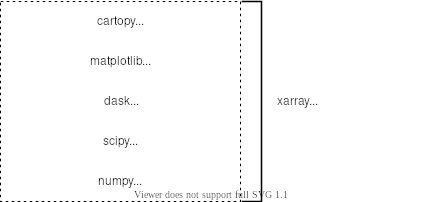
\includegraphics[scale=0.85]{01-pyaos-stack.png}} 
	
\end{frame}

\begin{frame}{Libraries for GIS}
	
	\only<1>{\centering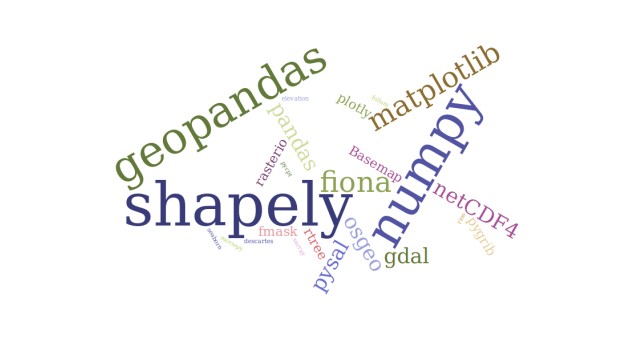
\includegraphics[scale=0.53]{gis_libs.png}} 
	
\end{frame}

\begin{frame}{Libraries gives kind of Neo's vision on Climate Data}
	
	\only<1>{\centering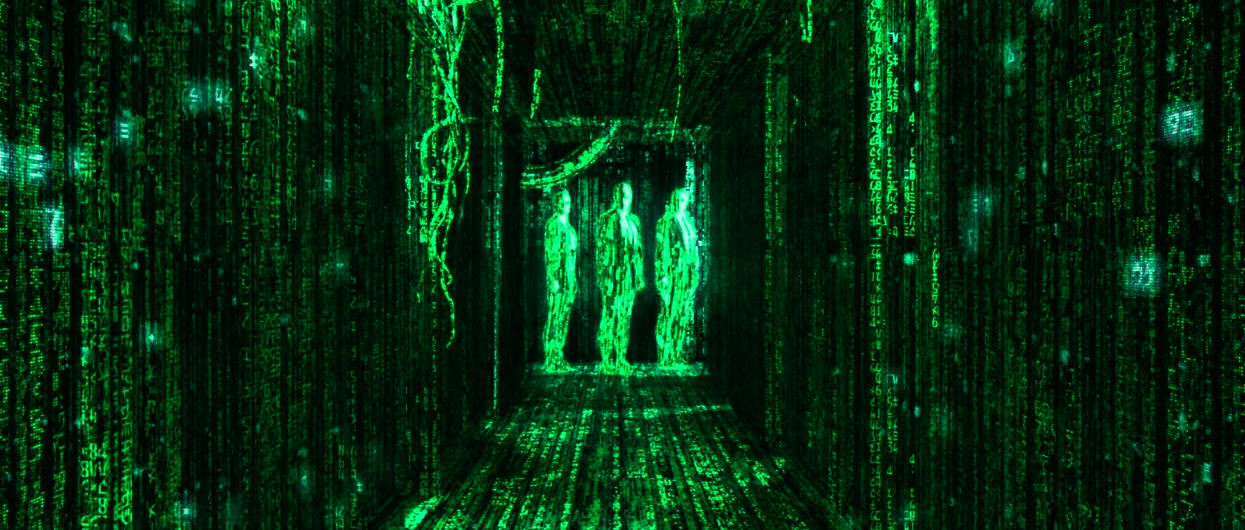
\includegraphics[scale=0.33]{neo_vision.png}} 
	
\end{frame}


\begin{frame}{Python libraries for raster operations}
	%\Fontvi
	\begin{beamerboxesrounded}{}
		\begin{itemize}
			\item rasterio gives tools to read geotiff
			\item Convert the satellite imagery into simple numpy array
			\item Several algorithm to clean and detect features in imagery
		\end{itemize}
	\end{beamerboxesrounded}
\end{frame}


\begin{frame}{Python libraries for vector operations}
	\begin{beamerboxesrounded}{}
		\begin{itemize}
			\item Geopandas to read the shape file
			\item Shapely to perform various vector operation
			\item Rtree index for spatial indexing of large data sources
		\end{itemize}
	\end{beamerboxesrounded}
\end{frame}

\section[Data exploration and visualization ]{Data exploration and visualization}

\begin{frame}{Data exploration and visualization}
	\begin{beamerboxesrounded}{Contents based on }
		\begin{itemize}
			\item https://carpentries-lab.github.io/python-aos-lesson/
		\end{itemize}
	\end{beamerboxesrounded}
	\begin{beamerboxesrounded}{To work on}
		\begin{itemize}
			\item Import the xarray library and use the functions it contains
			\item Convert precipitation units to mm/day
			\item Calculate and plot the precipitation climatology
			\item Use the cmocean library to find colormaps designed for ocean science
		\end{itemize}
	\end{beamerboxesrounded}
\end{frame}


\section[Functions and Command lines programs]{Functions and Command lines programs}

\begin{frame}{Functions and Command lines programs}
	\begin{beamerboxesrounded}{To work on}
		\begin{itemize}
			\item Define a function that takes parameters
			\item Use docstrings to document functions
			\item Break our existing plotting code into a series of small, single-purpose functions
			\item Use the argparse library to manage command-line arguments in a program
			\item Structure Python scripts according to a simple template
		\end{itemize}
	\end{beamerboxesrounded}
\end{frame}

\section[Demo Programs]{Demo Programs}

\begin{frame}{Demo Programs}
	\begin{beamerboxesrounded}{To work on}
		\begin{itemize}
			\item Read GFS data and plot maps
			\item Wind animation from GFS data
		\end{itemize}
	\end{beamerboxesrounded}
\end{frame}


\section[]{}

\begin{frame}{}
	\Large
	
	Thank you
	
\end{frame}   